\chapter{Introducción}
\label{ch:introduccion}

El Sol por excelencia es la fuente de energía electromagnética más potente y abundante en nuestro sistema planetario. El sol por si solo representa mas del 98\% de masa del Sistema Solar, la distancia del Sol a la Tierra es aproximadamente de 150 millones de kilómetros, su luz demora más de 8 minutos en alcanzar nuestro planeta y además produce 760.000 veces la cantidad de energía consumida en todo el planeta en un año. Tan solo una pequeña porción de toda la energía que esta estrella emite al espacio es recibida por nuestro planeta y solo una pequeña porción de la energía que llega es aprovechada de manera efectiva. La energía que recibimos del sol es causante de la mayoría de las condiciones climáticas que posee el planeta tierra y que permiten la existencia de la vida como la apreciamos diariamente.\\

\begin{figure}[h!]
        \centering
        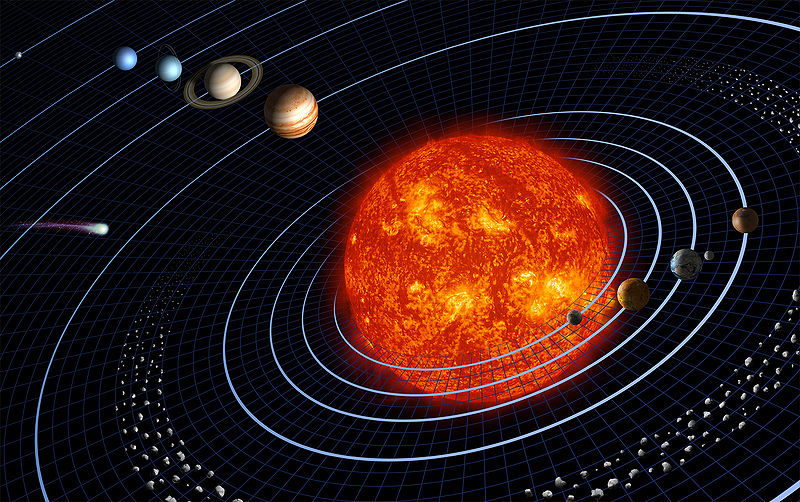
\includegraphics[scale=0.35]{images/solarSis}
        \caption{Sistema Solar}
\end{figure}

Esta Memoria tiene por objetivo desarrollar un sistema informático, que compuesto del software y los instrumentos de precisión adecuados, permita a la RedSolLac exponer a la comunidad, información respecto de la producción de energía fotovoltaica de Latinoamérica y el Caribe.\\ 
	
Fundación Chile, es una fundación de carácter privado sin fines de lucro, que se dedica a la creación de valor que aporte al desarrollo del país, dentro de sus áreas de desarrollo encontramos la gerencia de Energía y Cambio Climático que a su vez posee un área de Energía Solar. Dentro del área de Energía Solar se encuentran en ejecución, encargado por el Banco Interamericano de Desarrollo (\gloss{bid}), un proyecto para la creación de una red solar para Latinoamérica y el Caribe, RedSolLac\cite{redSolLac:1}. El objetivo de esta red es generar a corto y mediano plazo una red de coordinación en la región que sea referente en temas de energía solar y que potencie el desarrollo, la investigación y la utilización de la energía solar.\\
 
Como una primera etapa del desarrollo de esta comunidad, se encuentra la integración de estaciones de medición instaladas y por instalar en diferentes regiones de Chile, las cuales generarán una importante data que pasará a formar parte de una base de datos de radiación de energía solar. Estos datos deben estar disponible a toda la comunidad de manera abierta para aportar en el desarrollo de estas energías.\\

Durante el desarrollo de esta memoria se implementa una estacione de medición y se desarrollara un software que permita difundir los datos capturados así como herramientas que ayuden en la toma de decisiones respecto de la instalación de sistemas productores de energía fotovoltaica a todo nivel de actividad. En los primeros capítulos se abarcaran los alcances de esta memoria y temas introductorios a la energía solar, mientras que en los siguientes capítulos se describe de manera detallada las herramientas desarrolladas y el proceso de implementación, finalmente se expondrán los resultados de una fase de captura de datos y prueba del sistema.
